\chapter{Laboratorio 3}

Il primo circuito analizzato è un rettificatore a doppia semionda di precisione (\Fig\ref{fig:circuito_1}). Grazie all'utilizzo di due amplificatori operazionali ed un diodo, è possibile eliminare i problemi relativi al rettificatore a doppia semionda visto nella precedente esperienza di laboratorio, dove veniva utilizzato un unico amplificatore operazionale e due diodi. Per questo circuito sono stati utilizzati due amplificatori operazionali \textit{general-purpose} \textbf{\textmu A741} \url{https://www.ti.com/lit/ds/symlink/ua741.pdf}.
\begin{figure}[ht!]
	\centering
	\begin{minipage}{.45\textwidth}
		\scalebox{.73}{
			\begin{circuitikz}
				\draw (0,-.5) node[ground]{};
				\draw (0,1) coordinate (vin) to[sV=$v_{in}$] (0,-.5);
				\draw (vin) -- ++(0,1);
				\draw (0,2) -- ++(.32,0) to[R=$R_2$] ++(3,0);
				\draw (3,2) to (4,2);
				\draw (3.7,2) node[op amp, anchor=-](oa){\texttt{\textmu A741}};
				\draw (oa.down) ++(.5,.2) node[below]{$A1$};
				\draw (oa.up) -- ++(0, .3) node[vcc]{$+E$};
				\draw (oa.down) -- ++(0,-.3) node[vee]{$-E$};
				\draw (vin) to[R=$R_1$] (oa.+);
				\draw (1.32,-2) node[op amp, anchor=-](oa2){\texttt{\textmu A741}};
				\draw (oa2.down) ++(.5,.2) node[below]{$A2$};
				\draw (oa.+) -- ++(0,-1) to[D=$D_1$, invert] (oa2.out-|oa.+) to[short, -o] ++(0,0) ++(0,-.1) node[below]{$v_{out2}$};
				\draw (oa2.-) -- ++(0,2) -- ++(2.4,0);
				\draw (oa2.up) -- ++(0, .3) node[vcc]{$+E$};
				\draw (oa2.down) -- ++(0,-.3) node[vee]{$-E$};
				\draw (oa2.+) -- ++(0,-.3) node[ground]{};
				\draw (oa.up) -- ++(0, .3) node[vcc]{$+E$};
				\draw (oa.down) -- ++(0,-.3) node[vee]{$-E$};
				\draw (oa2.+) to[short,-o] ++(0,0) node[left]{$v^2_+$};
				\draw (oa2.-) to[short,-o] ++(0,0) node[left]{$v^2_-$};
				\draw (oa.+) to[short,-o] ++(0,0) node[above]{$v^1_+$};
				\draw (oa.-) to[short,-o] ++(0,0) node[above]{$v^1_-$};
				\draw (3,2) -- ++(0,2) coordinate(C) to[R=$R_3$] ++(3.08,0) (C-|oa.out) coordinate(Co) to[short, -] (oa.out) -- ++(1,0) coordinate(vmin) to [short, -o] ++(1,0) ++(.1,.1) node[above]{$v_{out}$};
				\draw[thick] (-1,-4.5) rectangle (9,5);
			\end{circuitikz} 
		}
	\end{minipage}\qquad
	\begin{minipage}{.45\textwidth}
		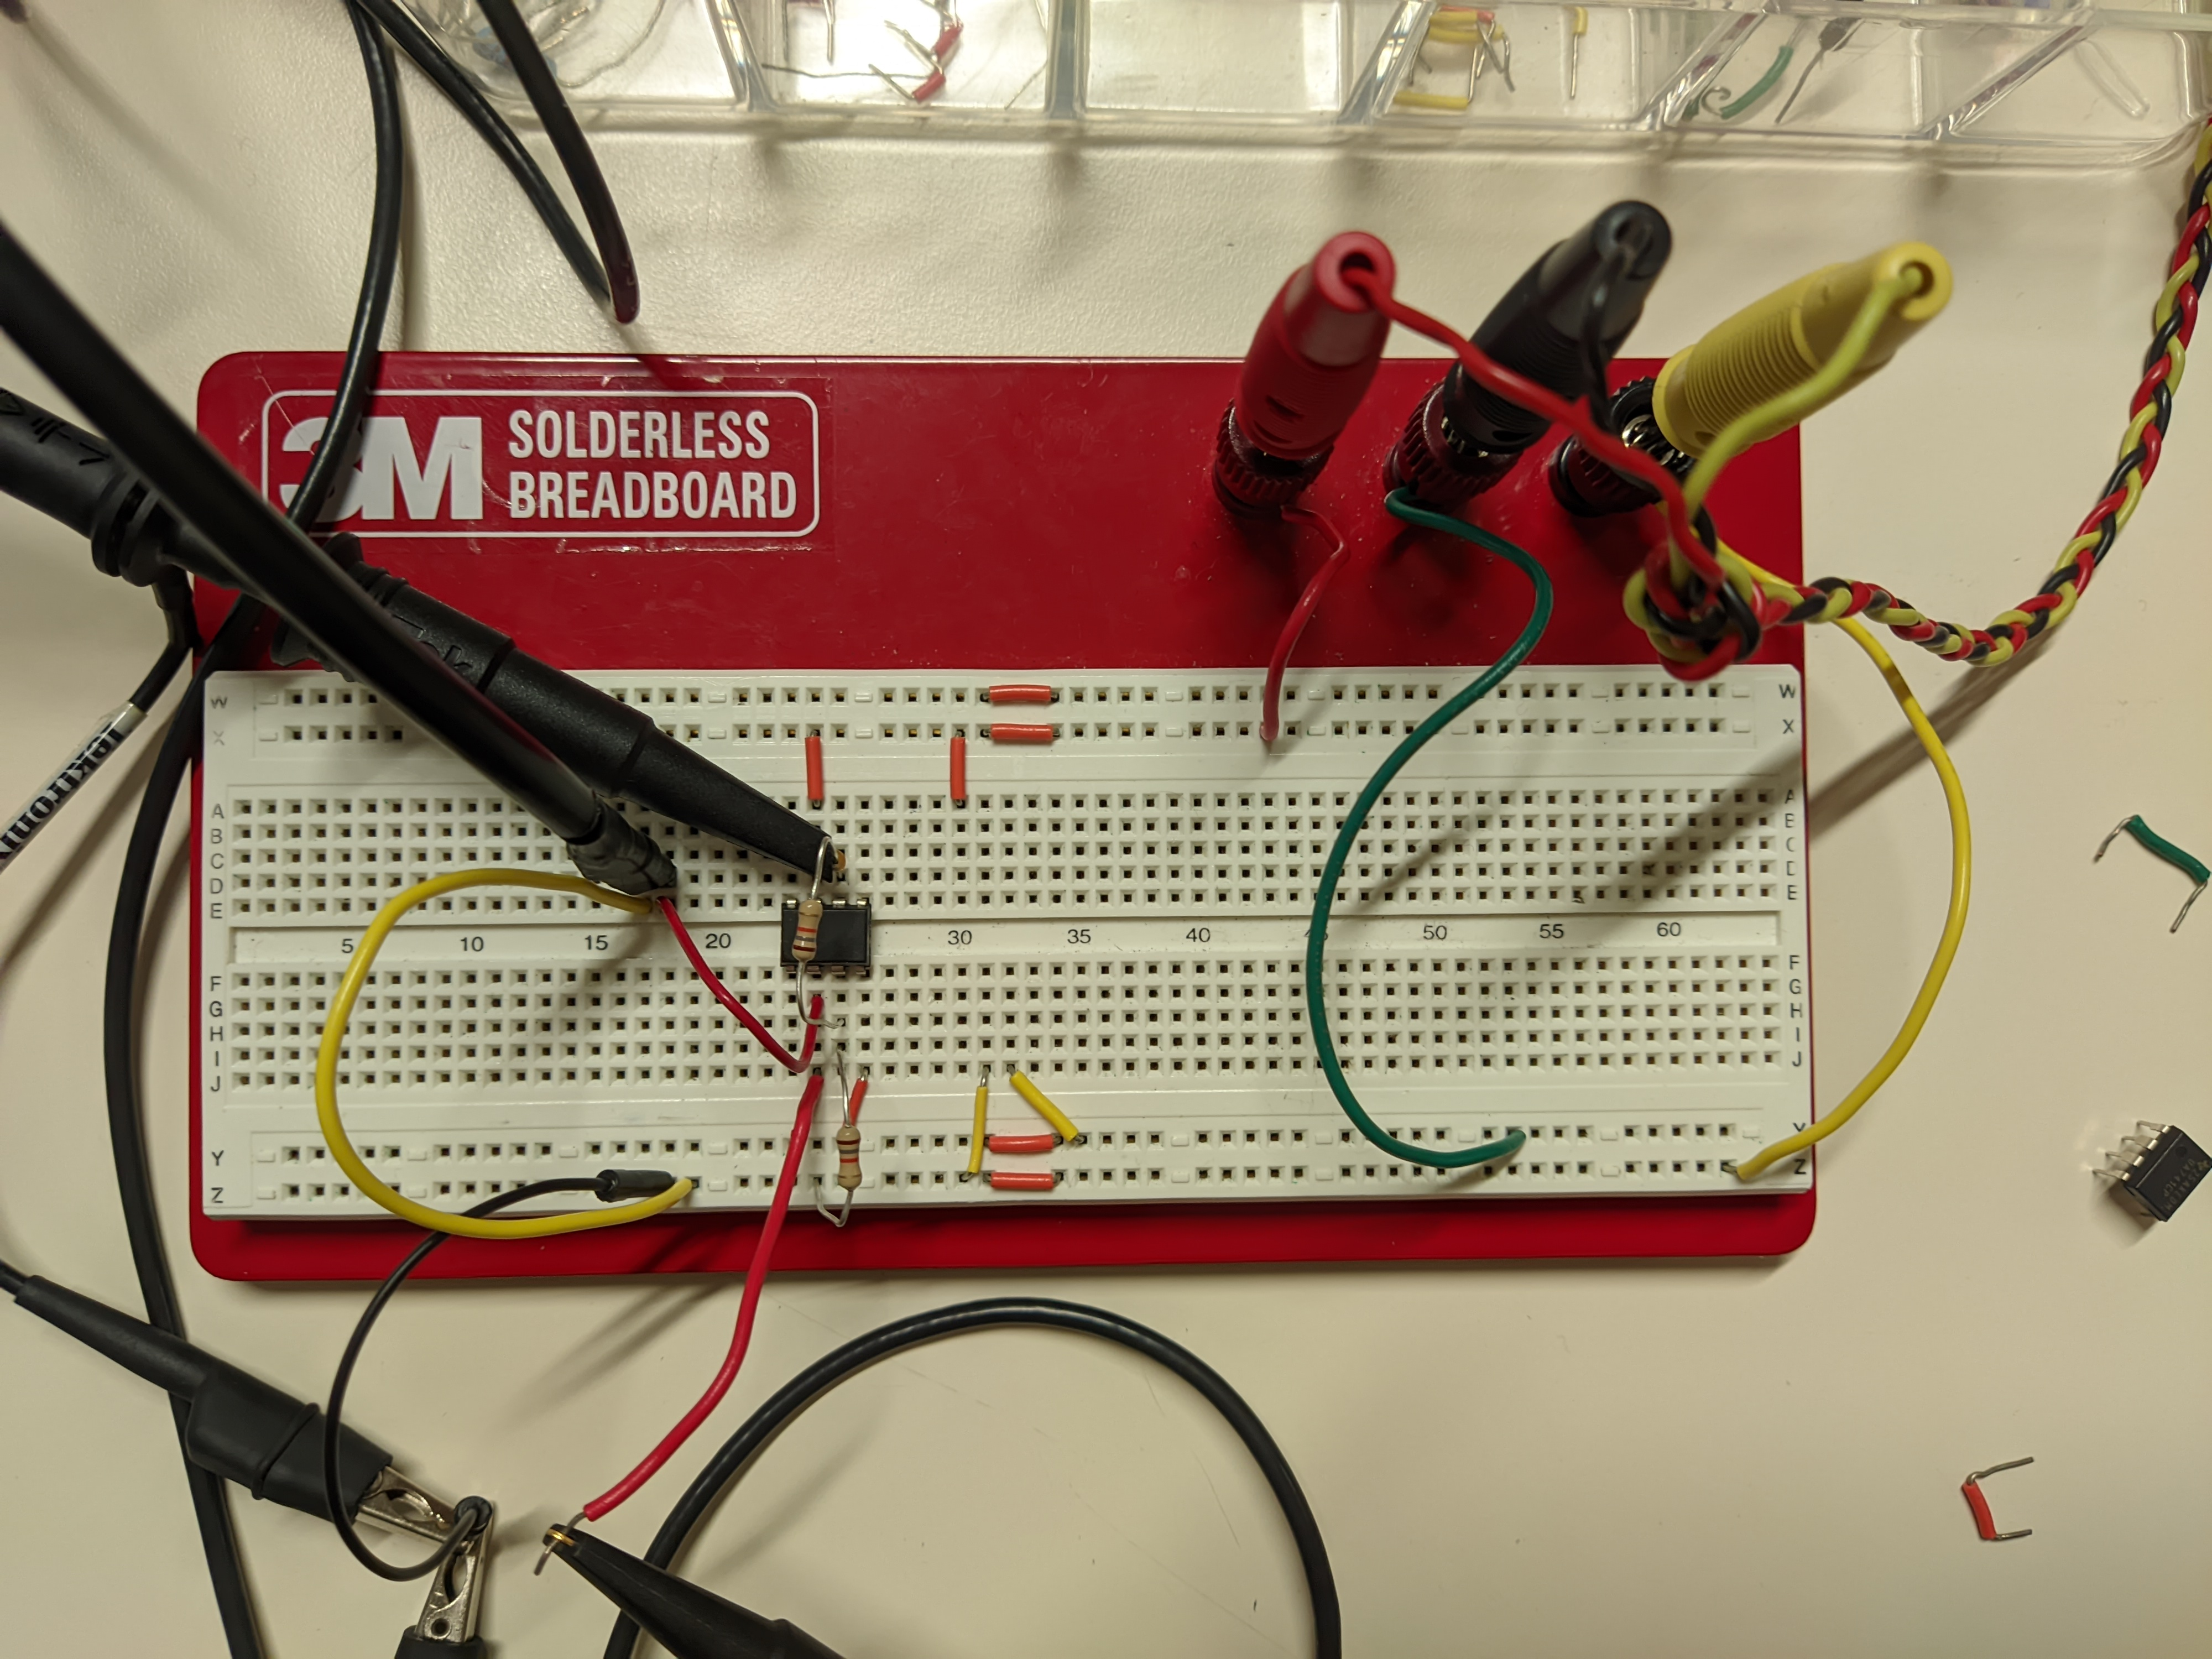
\includegraphics[width=\linewidth]{./ImageFiles/Laboratorio 3/CIR11.jpg}
	\end{minipage}
	\caption{Schema circuitale del raddrizzatore a doppia semionda e foto del circuito realizzato.}
	\label{fig:circuito_3}
\end{figure}

\noindent
Per studiare il comportamento del sistema è necessario analizzare come si comporta il diodo al variare della tensione di ingresso $v_{in}$:
\begin{itemize}
	\item $v_{in} \geq 0$: si ipotizza inizialmente che il diodo sia acceso. Allora, $A2$  è in retroazione negativa. Di conseguenza vale il principio di cortocircuito virtuale e quindi il nodo $v_{+}^1$ è a massa. Se questo fosse vero, la corrente dovrebbe percorrere la resistenza $R1$ da sinistra verso destra\todo{Nominiamo le resistenze anche se hanno lo stesso valore se non spiegare il circuito è un casino. le nominiamo dal basso all'alto, quindi R1 è quella più in basso. Marco: Dovrebbe essere giusto, verificate}. Tuttavia, ciò non è possibile, perchè i morsetti dell'amplificatore operazionale non assorbono corrente e il diodo non permette il passaggio di corrente in quel verso. Quindi, l'ipotesi che il diodo sia acceso non è corretta e assumiamo che il diodo è spento. Questo significa che l'amplificatore $A2$ non è retroazionato. Allora, in $R1$ non può scorrere corrente e la tensione sul nodo $v_{+}^1$ è pari a $v_{in}$. Ma questo implica che anche la tensione sul nodo $v_{-}^1$ sia pari a $v_{in}$. Di conseguenza, non scorre corrente neanche in $R2$ e quindi nemmeno in $R3$. Allora, la tensione $v_{out} = v_{in}$;
	\item $v_{in} < 0$: si ipotizza che il diodo sia acceso, quindi $A2$ è retroazionato negativamente. Il nodo $v_{+}^2$ è connesso ad una massa virtuale e quindi la corrente scorre nella resistenza $R1$ da destra a sinistra, dato che $v_{in} < 0$. Tale corrente può provenire dal diodo e questo verifica l'ipotesi iniziale. Se $v_{+}^1$ è a massa, lo è anche $v_{-}^1$, quindi $A1$ è in configurazione invertente. Se $R2 = R3$, il guadagno dell'amplificatore invertente è pari a 1 e $v_{out} = -v_{in}$.
\end{itemize}
Di conseguenza, questo circuito rettifica entrambe le semionde e eliminando il problema dello \text{shift} di tensione causato dalla tensione di polarizzazione del diodo. Nella figura \todo{inserire figura 01} è possibile verificare il comportamento del circuito.

\todo{inserire tabella con valori effettivi e misurati anche del diodo come nelle scorse relazioni e aggiungere indicazioni tensione +E e -E}

\noindent
Inoltre, si può verificare la caratteristica ingresso-uscita del circuito analizzando il grafico XY generato dall'oscilloscopio \todo{inserire figura 00}. Questo grafico mostra la tensione di uscita (asse delle ordinate) in funzione della tensione in ingresso (asse delle ascisse) e rappresenta una funzione di valore assoluto: infatti, il compito di un rettificatore è quello di lasciare inalterato il segnale in ingresso se positivo ed invertire il segnale in ingresso se negativo.

\noindent
Successivamente si è analizzato il comportamento in frequenza del circuito, effettuando delle misure di $v_{in}$ e $v_{out}$ con l'oscilloscopio, variando la frequenza della sinusoide in ingresso. \todo{inserire foto 01,03,04,05}
\`E possibile notare che dalla frequenza di \SI{1}{\kilo\hertz} l'uscita presenta un ritardo sul fronte di salita e il circuito dai \SI{10}{\kilo\hertz} non funziona più come un raddrizzatore. Questo comportamento è legato allo \textit{slew rate} dell'amplificatore \textit{A2}. Infatti, quando il diodo è spento \textit{A2} non è più in retroazione e l'uscita $v_{out}^2$ satura alla tensione di saturazione negativa (poiché $v_+^2$ è a massa e $v_-^2=v_{in}>0$).\todo{aggiungere immagine 02} Il nodo $v_{out}^2$ dovrà quindi passare immediatamente dalla tensione -E a \SI{0}{\volt}. Dal datasheet si ricava che lo \textit{slew rate} del \textbf{\textmu A741} è pari a \SI{0.5}{\volt\per\micro\second}. Si è cercato di stimare questo parametro delle misure effettuate \todo{inserire figura 06}. Il valore stimato è di circa $\frac{\SI{8.11}{\volt}}{\SI{20.0}{\micro\second}}=\SI{0.41}{\volt\per\micro\second}$, compatibile con le indicazioni presenti sul datasheet.

\clearpage
Il secondo circuito analizzato è chiamato \textbf{Trigger di Schmitt} e svolge la funzione di comparatore con isteresi. \todo{inserire foto circuito e schema}
Come si può osservare nel circuito, il segnale di ingresso $v_{in}$ viene applicato al morsetto invertente di un amplificatore operazionale (nel nostro caso si è utilizzato il \textbf{\textmu A741}), retroazionato positivamente grazie alle resistenze R\sub{1} e R\sub{2}. Per cui, non è più valido il principio di cortocircuito virtuale tra V\super{+} e V\super{-}, poiché non è più presente una retroazione negativa. Per cui, l'uscita $v_{out}=A(v^+-v^-)$, con A pari al guadagno dell'amplificatore operazionale, e il circuito si comporta come un comparatore. Infatti, supponendo un guadagno molto alto (idealmente tendente all'infinito), accade che:
\begin{itemize}
	\item se $v^+-v^->0$, allora $v_{out}=+E$;
	\item se $v^+-v^-<0$, allora $v_{out}=-E$.
\end{itemize}
Tuttavia, nel \textit{Trigger di Schmitt} la soglia alla quale l'uscita passa dalla tensione di saturazione positiva a quella negativa è diversa rispetto a quella presentata di un normale comparatore. Le resistenze R\sub{1} e R\sub{2} definiscono un partitore di tensione per cui $v^+=\frac{R_1}{R_1+R_2}v_{out}$. Supponendo che inizialmente la tensione $v_{in}$ sia pari a -E, di conseguenza l'uscita $v_{out}$ saturerà alla tensione +E (in quanto $v_{in}$ è applicata al morsetto invertente). Infatti, la tensione al nodo $v^+$ sarà pari a $v^+=\frac{R_1}{R_1+R_2}(+E)=V_H^+$ e se $R_1=R_2$ risulta che $V_H^+=\frac{1}{2}(+E)$. Per cui, fintanto che la tensione $v_{in}$ sarà minore della tensione $V_H^+$, l'uscita resterà alla tensione +E. Quando si avrà che $v_{in}>V_H^+$, l'uscita si porterà alla tensione di saturazione negativa -E e rimarrà tale fino a quando $v_{in}<V_L^+=\frac{R_1}{R_1+R_2}(-E)\overset{\mathrm{R_1=R_2}}{=}V_L^+=\frac{1}{2}(-E)$. 

\noindent
Riassumendo, in uscita si avrà un'onda quadra che commuta tra la tensione +E e -E, con \textit{duty-cycle} regolato dal periodo del segnale in ingresso

\todo{magari inserire un grafico fatto tipo a mano su onenote per esempio delle soglie che magari è più pratico?}

\todo{continuare spiegazione }

\todo{inserire valori resistenze reale}
\todo{inserire spiegazione delle differenze con i comparatori normali}
\todo{inserire caratteristica ingresso uscita con anche la foto oscilloscopio}